\chapter{In che cosa differisce l’allineamento globale dal locale e dal semi-globale anche in termini
di calcolo dello stesso}

Siano $V = v_1 v_2 \ldots v_n$ e $W = w_1 w_2 \ldots w_m$ due stringhe di lunghezza $n$ e $m$ definite su un alfabeto $\Sigma$. Si indica con $-$ il simbolo di gap
e con $\delta : (\Sigma \cup \{-\}) \times (\Sigma \cup \{-\}) \rightarrow \mathbb{N}$ una funzione di costo che assegna un costo a ogni coppia di simboli (compresi i gap), in particolare:
\begin{itemize}
    \item $\delta(v_i,w_j)=k$ se $v_i=w_j$ (match)
    \item $\delta(v_i,w_j)=s$ se $v_i \neq w_j$ (mismatch)
    \item $\delta(v_i,-)=\delta(-,w_j)=d$
\end{itemize}

Un allineamento tra $V$ e $W$ è una matrice $A$ di dimensione $2 \times k$ (con $k \geq \max(n,m)$) 
ottenuta inserendo eventualmente i gap nelle sequenze,
in modo tale che, eliminando i gap dalla prima riga, si ottiene $V$,
ed eliminando i gap dalla seconda riga, si ottiene $W$.
Ogni colonna di $A$ rappresenta un match, mismatch, inserzione o delezione.
Il punteggio di allineamento è dato dalla somma dei punteggi delle singole colonne:
\begin{equation}
    \text{C}(A) = \sum_{i=1}^{k} \delta(A_{1,i}, A_{2,i})
\end{equation}

Per calcolare un allineamento ottimo si usa una griglia di edit di dimensione
$(n+1) \times (m+1)$, in cui $S(i,j)$ rappresenta lo score ottimo per allineare il prefisso $v[1..i]$ con il prefisso $w[1..j]$.

\paragraph{Allineamento Globale}

L'\textbf{allineamento globale} di due sequenze $V$ e $W$ è un allineamento che considera entrambe le sequenze nella loro interezza.
Quindi l'obiettivo è trovare la matrice di allineamento $A$ di score ottimo
tra tutta la sequenza $V$ e tutta la sequenza $W$.

Nel calcolo tramite programmazione dinamica, $S(i,j)$ rappresenta lo score
ottimo di allineamento globale fra il prefisso $V_i$ e il prefisso $W_j$.

I \textbf{casi base} sono:
\begin{itemize}
    \item $S(0,0)=0$
    \item $S(i,0)= i \cdot d$
    \item $S(0,j)= j \cdot d$
\end{itemize}

Dove $d$ è il costo dell'inserimento di un gap. Infatti, per allineare un prefisso non vuoto con una stringa vuota, è necessario inserire solo gap, e ogni gap ha costo $d$.

Per $i > 0$ e $j > 0$ la ricorrenza è:
\begin{equation}
    S(i,j) = \operatorname{opt}
    \begin{cases}
        S(i-1,j-1) + \delta(v_i,w_j) & \text{(match/mismatch)} \\
        S(i-1,j) + \delta(v_i,-) & \text{(delezione)} \\
        S(i,j-1) + \delta(-,w_j) & \text{(inserzione)}
    \end{cases}
\end{equation}
dove $\operatorname{opt}$ indica l'operatore ottimo: $\min$ se si lavora con costi da minimizzare, $\max$ se si lavora con score da massimizzare.

Poiché si considerano entrambe le sequenze nella loro interezza, il punteggio ottimo si trova nel nodo finale $S(n,m)$.

La ricostruzione dell'allineamento avviene tramite backtracking, partendo da $S(n,m)$ e risalendo fino a $S(0,0)$, seguendo i movimenti che hanno portato al punteggio ottimo.
Si ottiene così la matrice di allineamento $A$.

\paragraph{Allineamento Locale}

Date due stringhe:
\[
V = v_1 v_2 \ldots v_n \quad \text{e} \quad W = w_1 w_2 \ldots w_m
\]
un \textbf{allineamento locale} consiste nel determinare il miglior allineamento globale
tra una sottostringa di $V$ e una sottostringa di $W$.

Quindi, a differenza dell'allineamento globale, non si vuole necessariamente
allineare tutta la sequenza $V$ con tutta la sequenza $W$, ma si vogliono
individuare le regioni più simili contenute nelle sequenze.

Formalmente, l'obiettivo è quindi di trovare due sottostringhe $V' = v_i v_{i+1} \ldots v_{i+k}$ e $W' = w_j w_{j+1} \ldots w_{j+k}$ (con $k \geq 0$) tali che lo score di
allineamento globale fra le due sottostringhe sia massimo fra tutte le possibili coppie di sottostringhe in $V$ e $W$.

Anche per l'allineamento locale si utilizza la griglia di edit $S$ di dimensione: $(n+1) \times (m+1)$,
dove però $S(i,j)$ rappresenterà il miglior score di allineamento globale
tra due sottostringhe che terminano rispettivamente in $v_i$ e $w_j$.

In altre parole, $S(i,j)$ non rappresenta lo score tra prefissi di $V$ e $W$,
ma il miglior score tra tutte le coppie di sottostringhe che terminano in $v_i$ e $w_j$.
Lo score dell'allineamento locale tra $V$ e $W$ sarà quindi il massimo valore
presente nella matrice $S$.

I \textbf{casi base} sono:
\begin{itemize}
    \item $S(0,0)=0$
    \item $S(i,0)=0$ per $0 \leq i \leq n$
    \item $S(0,j)=0$ per $0 \leq j \leq m$
\end{itemize}

A differenza dell'allineamento globale, qui non si inizializza la prima riga
e la prima colonna con il costo dei gap, in quanto le parti iniziali delle sequenze
che non appartengono alla sottostringa ottima possono essere ignorate. L'allineamento, infatti,
può iniziare in qualunque punto della matrice.

Per $i > 0$ e $j > 0$ la ricorrenza è:
\begin{equation}
    S(i,j) = \operatorname{opt} \begin{cases}
        0 \\
        S(i-1,j-1) + \delta(v_i,w_j)\\
        S(i-1,j) + \delta(v_i,-) \\
        S(i,j-1) + \delta(-,w_j)
    \end{cases}
\end{equation}

Il primo caso, con punteggio $0$, è la differenza principale rispetto
all'allineamento globale. Nel caso classico con score da massimizzare, se tutte le opzioni di allineamento hanno un punteggio negativo, è preferibile non allineare nulla,
quindi interrompere l'allineamento corrente e iniziare un nuovo allineamento a partire dalla cella successiva.

Una volta riempita la matrice $S$, lo score ottimo dell'allineamento locale non si trova necessariamente in $S(n,m)$ ma è:
\[
    \max_{0 \leq i \leq n, 0 \leq j \leq m} S(i,j)
\]
cioè il massimo valore presente nella matrice.
\begin{figure}[H]
    \centering
    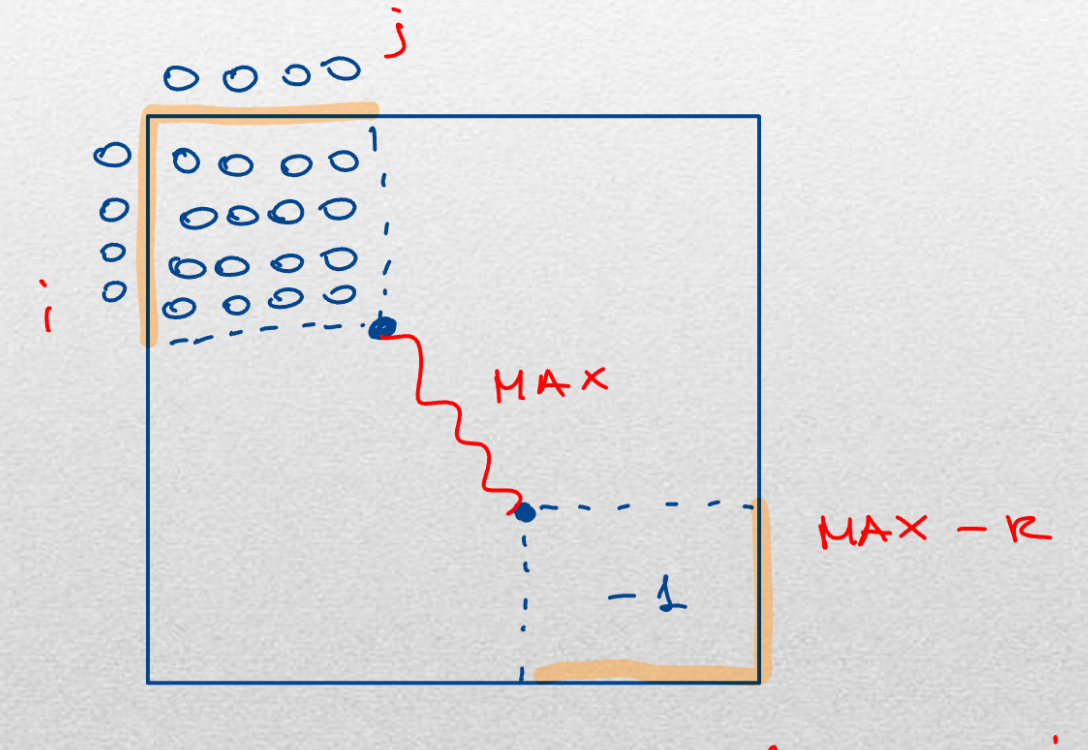
\includegraphics[width=0.7\textwidth]{images/local_allignment.png}
    \caption{Allineamento locale: scelta della regione con score ottimo.}
    \label{fig:local-alignment}
\end{figure}

La ricostruzione dell'allineamento avviene tramite backtracking, partendo dalla cella che contiene il punteggio massimo.
Il backtracking procede a ritroso seguendo i movimenti che hanno portato al punteggio ottimo e si ferma quando raggiunge una cella con punteggio $0$, che rappresenta
l'inizio dell'allineamento locale ottimo.

\begin{figure}[H]
    \centering
    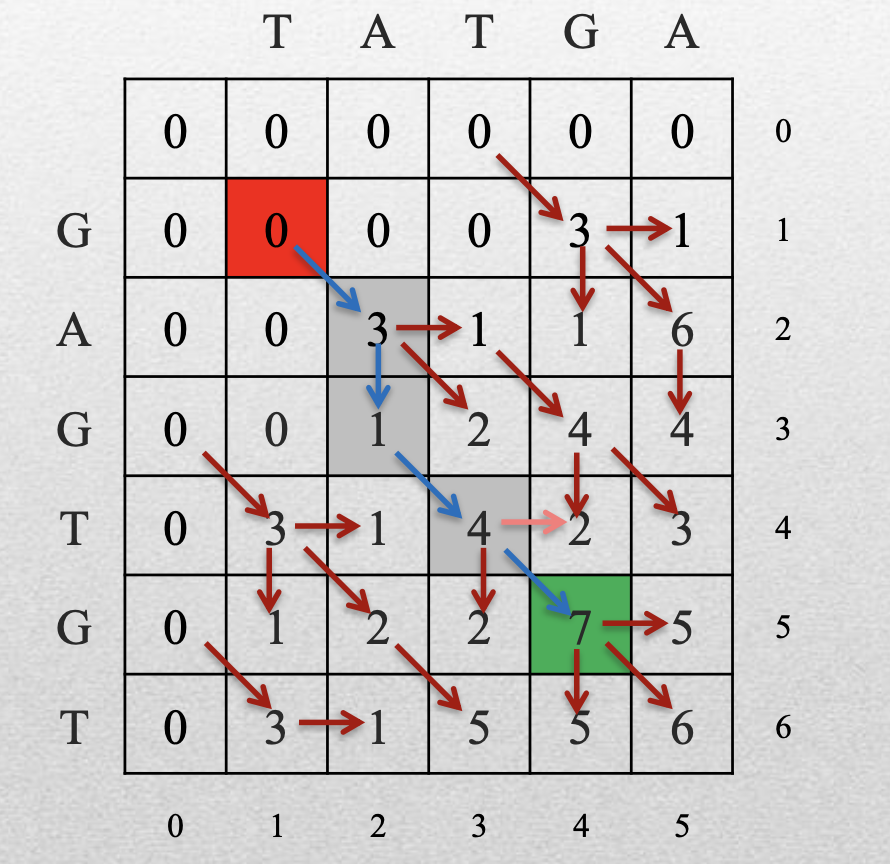
\includegraphics[width=0.7\textwidth]{images/back_locale.png}
    \caption{Backtracking nell'allineamento locale fino a una cella con punteggio $0$.}
    \label{fig:back-locale}
\end{figure}

\paragraph{Allineamento Semi-globale}

L'\textbf{allineamento semi-globale} di due sequenze
$V=v_1v_2\dots v_n$ e $W=w_1w_2\dots w_m$ è una famiglia di problemi di
allineamento in cui non si richiede necessariamente di allineare entrambe le
sequenze per intero, come nell'allineamento globale, ma non si cercano nemmeno
due sottostringhe completamente arbitrarie, come nell'allineamento locale.

L'idea generale è cercare un allineamento globale ottimo tra due porzioni
vincolate delle sequenze. Questo significa che il problema specifica che tipo
di porzione si può scegliere: un prefisso, un suffisso, una sottostringa,
oppure l'intera sequenza. Una volta scelta tale porzione, essa viene allineata
globalmente con l'altra porzione.

Quindi, in generale, l'allineamento semi-globale cerca un allineamento globale
ottimo tra $V[a..b]$ e $W[c..d]$,
dove però gli indici $a,b,c,d$ non sono completamente liberi come nel locale,
ma sono vincolati dal tipo di problema, in particolare:
\begin{itemize}
    \item se si cerca un prefisso di $V$, allora la porzione deve iniziare da
    $v_1$, quindi è del tipo $V[1..b]$;
    \item se si cerca un suffisso di $W$, allora la porzione deve terminare in
    $w_m$, quindi è del tipo $W[c..m]$;
    \item se si cerca una sottostringa di $V$, allora la porzione può iniziare
    e finire in posizioni interne, quindi è del tipo $V[a..b]$;
    \item se si considera tutta $W$, allora la porzione è fissata ed è
    $W[1..m]$.
\end{itemize}

La stessa cosa vale per la sequenza $W$.

Dal punto di vista del calcolo, anche l'allineamento semi-globale usa una
matrice dinamica $S$ di dimensione:
\[
    (n+1) \times (m+1)
\]

La ricorrenza interna è in genere la stessa dell'allineamento globale:
\[
    S(i,j)=\operatorname{opt}
    \begin{cases}
        S(i-1,j-1)+\delta(v_i,w_j)\\
        S(i-1,j)+\delta(v_i,-)\\
        S(i,j-1)+\delta(-,w_j)
    \end{cases}
\]

La differenza rispetto al globale sta nel fatto che non sempre l'ottimo viene
cercato nella cella finale $S(n,m)$. A seconda del tipo di porzione considerata,
lo score ottimo può essere cercato nell'ultima riga, nell'ultima colonna, in
tutta la matrice o in un'altra regione specifica.

Anche l'\textbf{inizializzazione} e il \textbf{punto di arresto del backtracking}
dipendono dal problema semi-globale considerato: le parti della sequenza che
possono essere ignorate non vengono penalizzate, mentre le parti che devono
essere effettivamente allineate vengono trattate come in un allineamento
globale.

\textbf{1. Prefisso di $V$ contro tutta $W$}

\[
    V[1..r] \quad \text{contro} \quad W[1..m]
\]

Lo score ottimo si cerca nell'ultima colonna:
\[
    \max_{0 \leq i \leq n} S(i,m)
\]
perché $W$ deve essere considerata interamente, mentre il prefisso di $V$ può
terminare in una qualunque posizione $i$.

\begin{figure}[H]
    \centering
    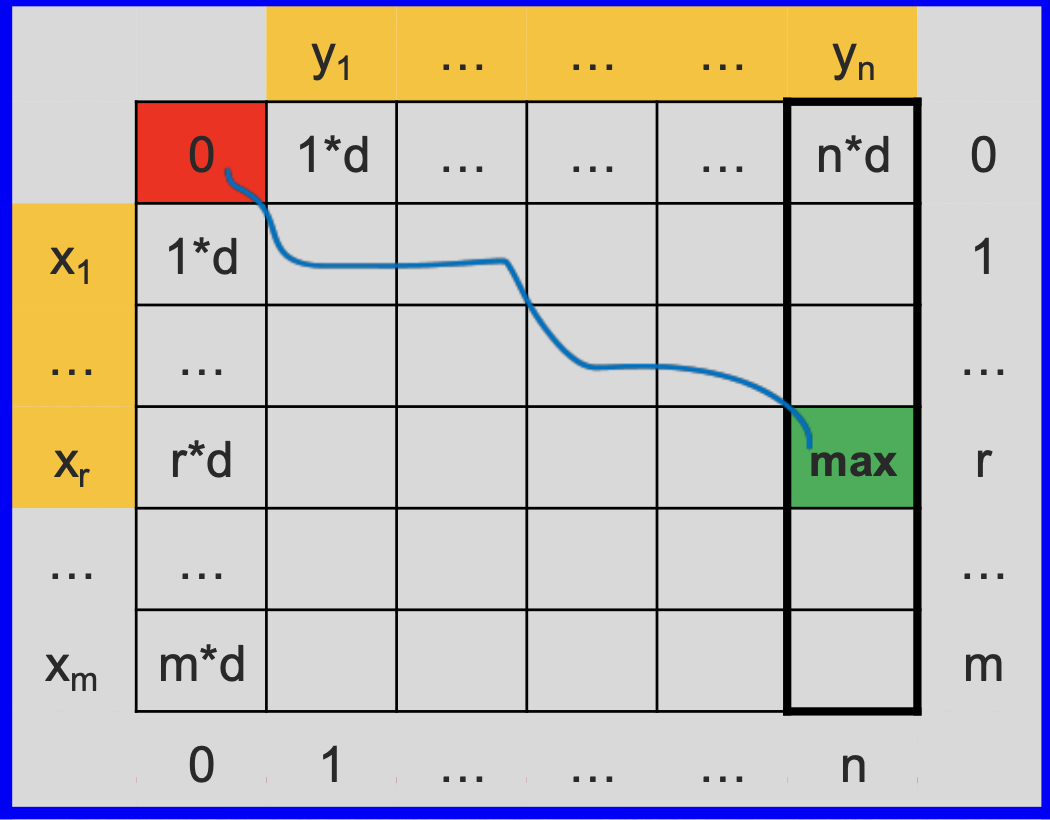
\includegraphics[width=0.6\textwidth]{images/preXvsY.png}
    \caption{Allineamento tra un prefisso di $V$ e tutta $W$.}
    \label{fig:semiglobale-prefisso-v-tutta-w}
\end{figure}

\textbf{2. Tutta $V$ contro prefisso di $W$}

\[
    V[1..n] \quad \text{contro} \quad W[1..c]
\]

Lo score ottimo si cerca nell'ultima riga:
\[
    \max_{0 \leq j \leq m} S(n,j)
\]
perché $V$ deve essere considerata interamente, mentre il prefisso di $W$ può
terminare in una qualunque posizione $j$.

\begin{figure}[H]
    \centering
    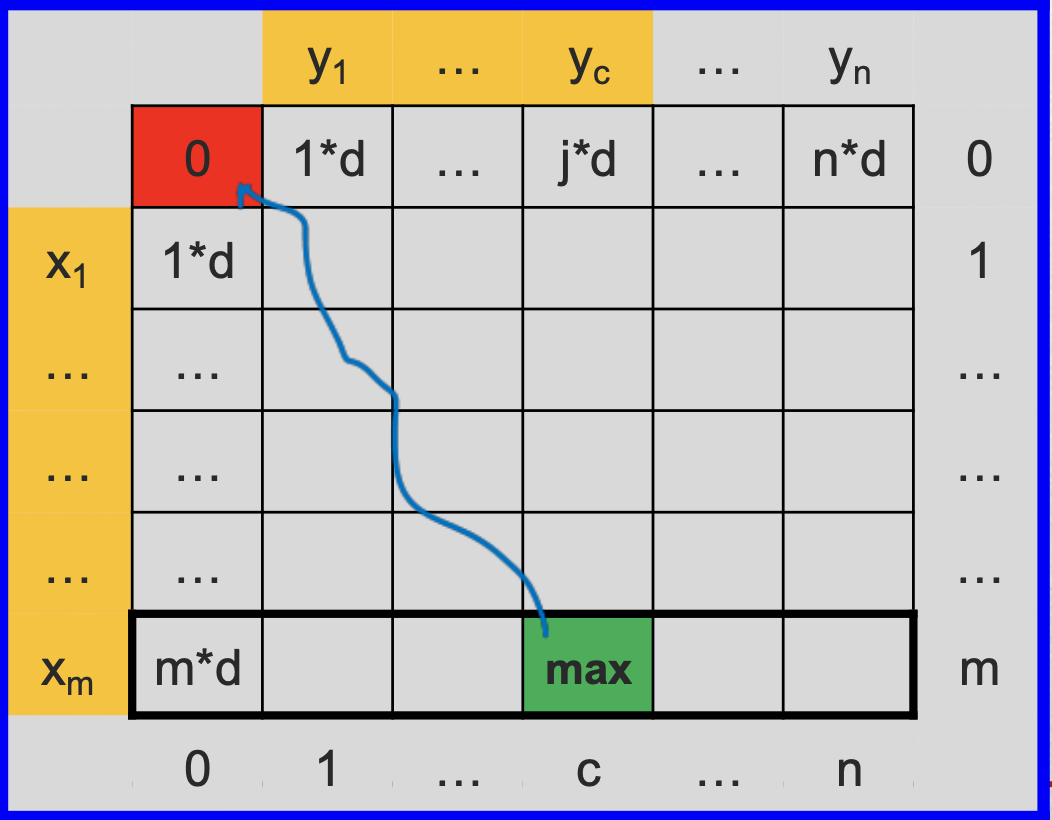
\includegraphics[width=0.6\textwidth]{images/XvsPreY.png}
    \caption{Allineamento tra tutta $V$ e un prefisso di $W$.}
    \label{fig:semiglobale-tutta-v-prefisso-w}
\end{figure}

\textbf{3. Prefisso di $V$ contro prefisso di $W$}

\[
    V[1..r] \quad \text{contro} \quad W[1..c]
\]

Lo score ottimo si cerca in tutta la matrice:
\[
    \max_{0 \leq i \leq n,\ 0 \leq j \leq m} S(i,j)
\]
perché entrambi i prefissi possono terminare in posizioni non fissate.

\begin{figure}[H]
    \centering
    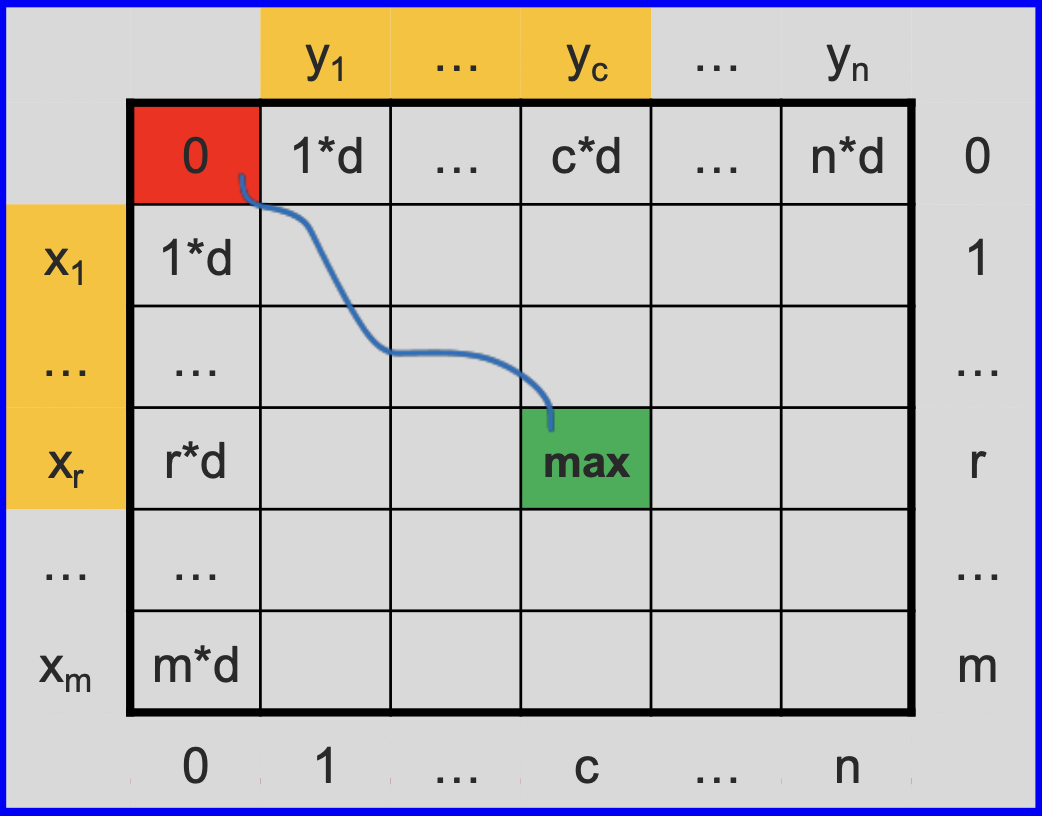
\includegraphics[width=0.6\textwidth]{images/preXvsPreY.png}
    \caption{Allineamento tra un prefisso di $V$ e un prefisso di $W$.}
    \label{fig:semiglobale-prefisso-v-prefisso-w}
\end{figure}

\textbf{4. Suffisso di $V$ contro suffisso di $W$}

\[
    V[a..n] \quad \text{contro} \quad W[c..m]
\]

Lo score ottimo si trova in:
\[
    S(n,m)
\]
perché entrambi i suffissi devono terminare alla fine delle rispettive sequenze.
Le parti iniziali non appartenenti ai suffissi possono invece essere ignorate.

\begin{figure}[H]
    \centering
    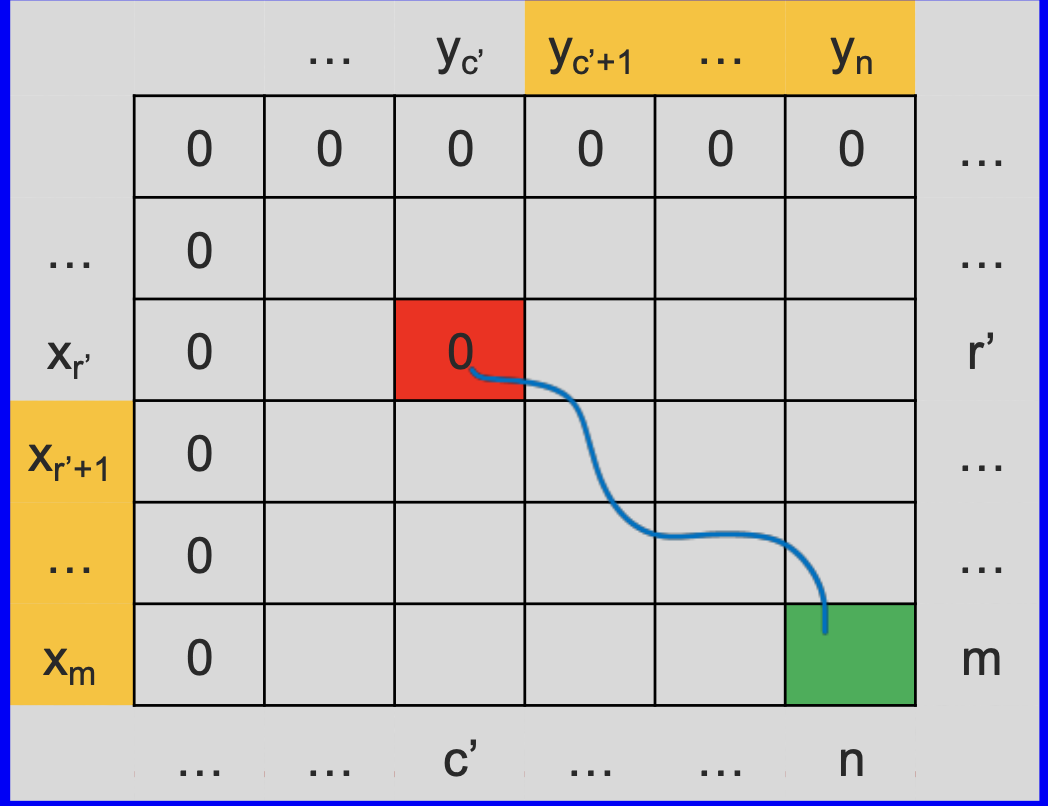
\includegraphics[width=0.6\textwidth]{images/suffXvsSuffY.png}
    \caption{Allineamento tra un suffisso di $V$ e un suffisso di $W$.}
    \label{fig:semiglobale-suffisso-v-suffisso-w}
\end{figure}

\textbf{5. Suffisso di $V$ contro prefisso di $W$}

\[
    V[a..n] \quad \text{contro} \quad W[1..c]
\]

Lo score ottimo si cerca nell'ultima riga:
\[
    \max_{0 \leq j \leq m} S(n,j)
\]
perché il suffisso di $V$ deve terminare in $v_n$, mentre il prefisso di $W$ può
terminare in una qualunque posizione $j$.

\begin{figure}[H]
    \centering
    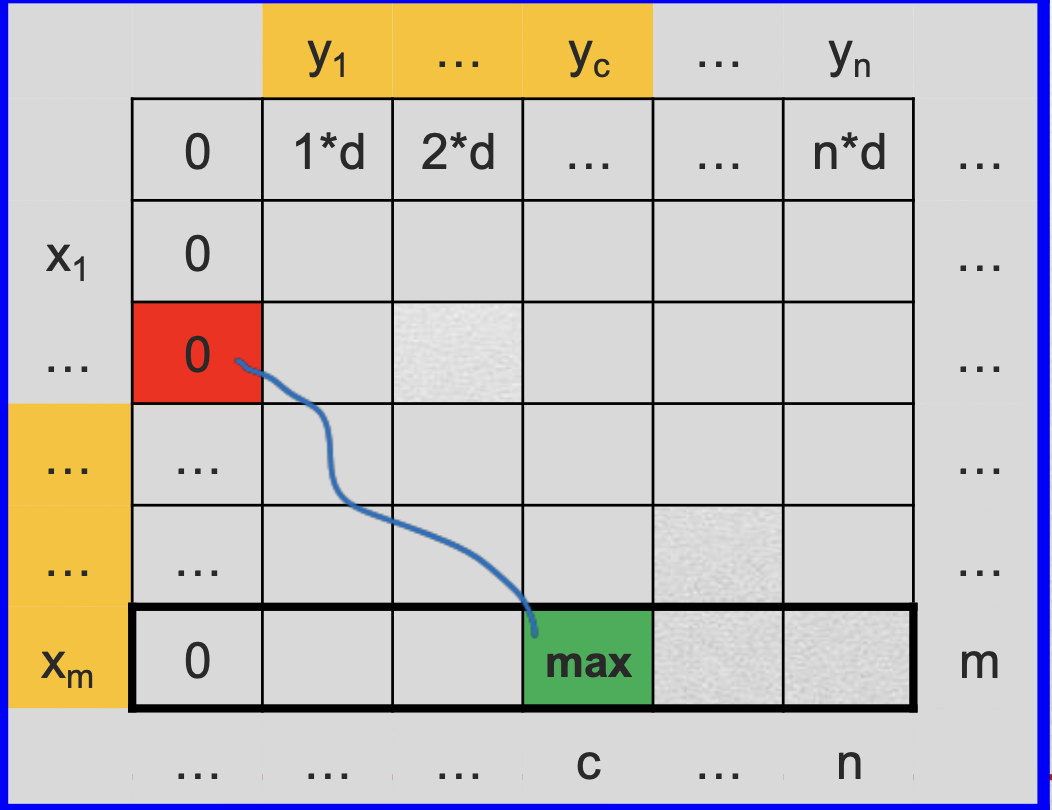
\includegraphics[width=0.6\textwidth]{images/SufPre.png}
    \caption{Allineamento tra un suffisso di $V$ e un prefisso di $W$.}
    \label{fig:semiglobale-suffisso-v-prefisso-w}
\end{figure}

\textbf{6. Sottostringa di $V$ contro tutta $W$}

\[
    V[a..b] \quad \text{contro} \quad W[1..m]
\]

Lo score ottimo si cerca nell'ultima colonna:
\[
    \max_{0 \leq i \leq n} S(i,m)
\]
perché $W$ deve essere usata tutta, mentre la sottostringa di $V$ può terminare
in una qualunque posizione $i$.

\begin{figure}[H]
    \centering
    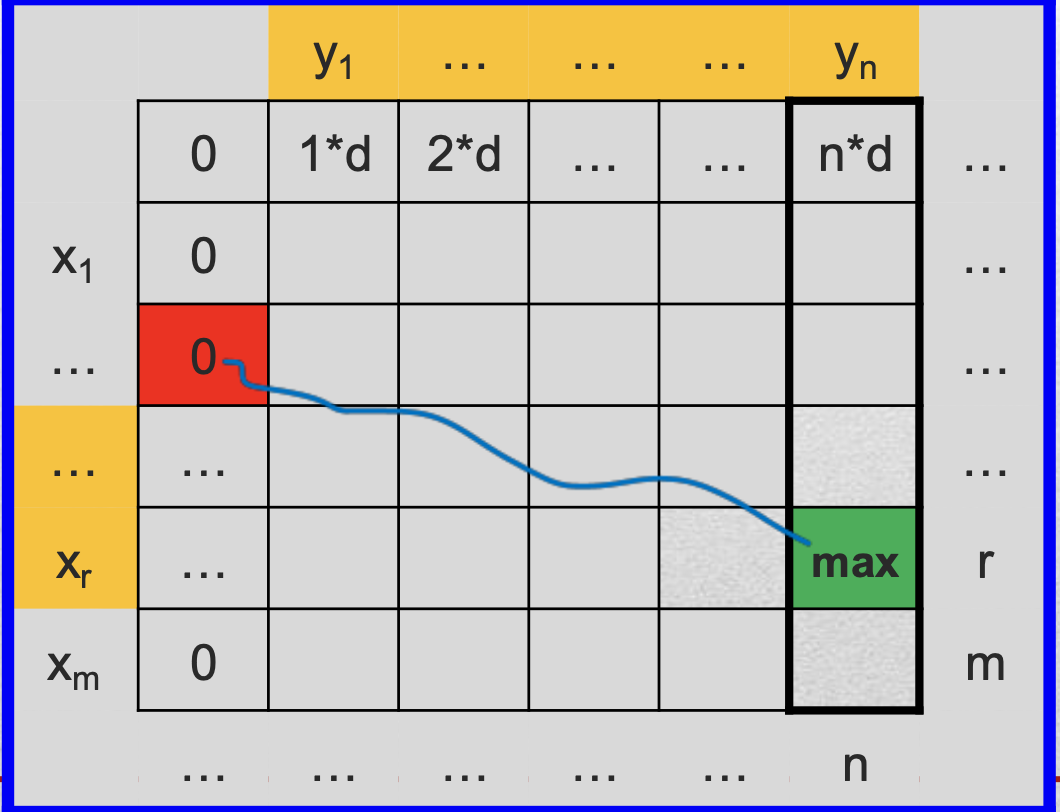
\includegraphics[width=0.6\textwidth]{images/subvsfull.png}
    \caption{Allineamento tra una sottostringa di $V$ e tutta $W$.}
    \label{fig:semiglobale-sottostringa-v-tutta-w}
\end{figure}
